\documentclass[12pt,a4paper]{article}
\usepackage{ctex}
\usepackage{geometry}
\usepackage{graphicx}
\usepackage{setspace}
\usepackage{listings}
\usepackage{xcolor}
\usepackage{hyperref}
\usepackage{float} 


\geometry{left=3cm,right=3cm,top=2.5cm,bottom=2.5cm}

% 代码样式
\lstset{
    language=Java,
    basicstyle=\ttfamily\small,
    keywordstyle=\color{blue}\bfseries,
    commentstyle=\color{green!50!black},
    stringstyle=\color{orange},
    showstringspaces=false,
    numbers=left,
    numberstyle=\tiny,
    breaklines=true,
    frame=single
}

\begin{document}

% ================= 封面 =================
\begin{titlepage}
\centering
\vspace*{2cm}

% 校徽 Logo 
\makebox[\textwidth][c]{%
  
\includegraphics[height=4cm]{fengmian.png}%
}


% 学院名称
{\zihao{1}\heiti 信息科学与工程学院}\\[1cm]

% 学年学期
{\zihao{4} 2025---2026 \kaishu学年第一学期}\\[1.5cm]

% 报告标题
\makebox[\textwidth][c]{%
  
\includegraphics[height=2cm]{shiyanbaogao.png}%
}
\\[2em] % 空行
% 实验基本信息表
\zihao{4} 
\renewcommand{\arraystretch}{1.8} % 表格行距
\begin{tabular}{rl}
\heiti 课程名称: & \underline{\makebox[18em][c]{\fangsong Java 编程技术}} \\
\heiti 实验名称: & \underline{\makebox[18em][c]{\fangsong 一个简单的控制台应用程序}} \\
\\[1em] % 空行
专  业  班  级: & \underline{\makebox[18em][c]{通信一班}} \\
学  生  学  号: & \underline{\makebox[18em][c]{202300120317}} \\
学  生  姓  名: & \underline{\makebox[18em][c]{陈都阳}} \\
实  验  时  间: & \underline{\makebox[18em][c]{2025年9月16日}} \\
\end{tabular}

\vfill
\end{titlepage}

% ================= 正文 =================
\section*{实验目的}
\begin{enumerate}
    \item 掌握安装 SDK 软件包、Eclipse 软件、EditPlus 编辑软件的方法。
    \item 掌握设置程序运行环境的方法。
    \item 掌握编写与运行程序的方法。
    \item 理解面向对象的编程思想。
\end{enumerate}

\section*{实验要求}
\begin{enumerate}
    \item 编写一个简单的控制台应用程序,该程序在命令行窗口输出两行文字:\\
    “Hello World!” 和 “We are students.”。
    \item 使用 Eclipse 编译运行,并截图实验结果。
    \item 使用命令行方式编译运行,并截图结果。
    \item 实验后回答相关思考问题。
\end{enumerate}

\section*{实验内容}

\subsection*{源代码}
\begin{figure}[H]
\centering
\begin{lstlisting}
// HelloWorld.java
public class HelloWorld {
    public static void main(String[] args) {
        System.out.println("Hello World!");
        System.out.println("We are students.");
    }
}
\end{lstlisting}
\caption{HelloWorld 源代码}
\end{figure}

\subsection*{实验过程与结果}

\begin{figure}[H]
\centering
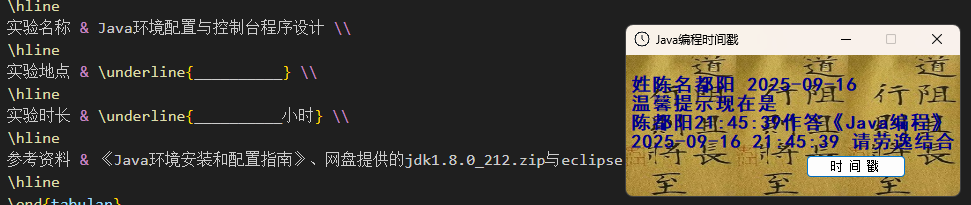
\includegraphics[width=0.8\textwidth]{eclipse_result.png}
\caption{Eclipse 运行结果}
\end{figure}

\begin{figure}[H]
\centering
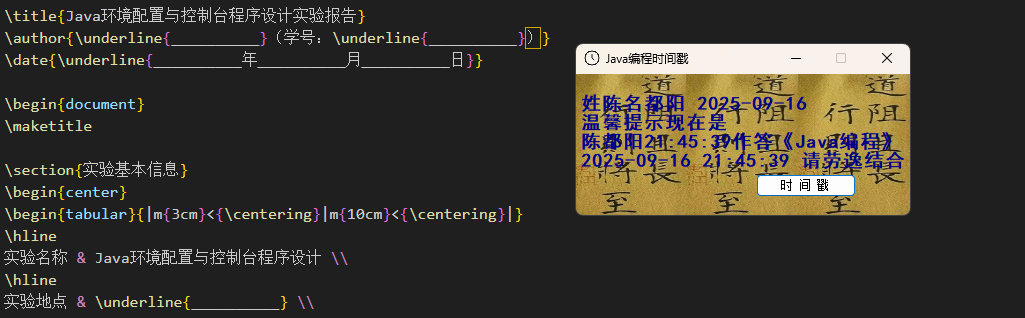
\includegraphics[width=0.8\textwidth]{cmd_result.png}
\caption{命令行运行结果}
\end{figure}

\section*{思考与分析}
\begin{enumerate}
    \item 编译器缺少大括号时,会提示 \texttt{'expected'} 错误。
    \item 编译器缺少分号时,会提示 \texttt{';' expected} 错误。
    \item 如果将 \texttt{System} 写成 \texttt{system},编译器会提示 \texttt{cannot find symbol}。
    \item 面向对象(OOP)是以对象为中心,强调对象之间的关系与交互;面向过程则是以步骤为中心,强调操作流程。  
    \item 例如五子棋:面向过程按步骤写函数(落子、判断输赢),面向对象则分为“玩家对象、棋盘对象、规则对象”,更模块化,扩展性更好。
\end{enumerate}

\section*{实验心得}
通过本次实验,我熟悉了 Java 开发环境的搭建,掌握了 Eclipse 和命令行编译运行 Java 程序的方法。同时,通过实验后的思考题,我加深了对面向对象与面向过程区别的理解。面向对象强调对象之间的协作,更适合大型系统的开发。

\end{document}
